\documentclass[a4paper, 12pt]{article}

\usepackage[sort&compress]{natbib}
\bibpunct{(}{)}{;}{a}{}{,} 

\usepackage{amsthm, amsmath, amssymb, mathrsfs, multirow, url, subfigure}
\usepackage{graphicx} 
\usepackage{ifthen} 
\usepackage{amsfonts}
\usepackage[usenames]{color}
\usepackage{fullpage}
\usepackage{setspace}
\usepackage{subfigure}

%\RequirePackage[OT1]{fontenc} 
%\RequirePackage[colorlinks]{hyperref}
%\RequirePackage{hypernat}


%\numberwithin{equation}{section} 

\graphicspath{ {./images/} } 

\theoremstyle{plain} 
\newtheorem{theorem}{Theorem}
\newtheorem{corollary}{Corollary}
\newtheorem{proposition}{Proposition}
\newtheorem{lemma}{Lemma}

\def\wl{\par \vspace{\baselineskip}}
\theoremstyle{definition}
\newtheorem{defn}{Definition}

\theoremstyle{remark} 
\newtheorem{remark}{Remark}
\newtheorem{example}{Example}
\newtheorem{assumption}{Assumption}
\newtheorem{condition}{Condition}


\newcommand{\prob}{\mathsf{P}} 
\newcommand{\E}{\mathsf{E}}

\newcommand{\probhat}{\widehat{\mathsf{P}}}

\newcommand{\bel}{\mathsf{bel}}
\newcommand{\pl}{\mathsf{pl}}
\newcommand{\mpl}{\mathsf{mpl}}

\newcommand{\GG}{\mathbb{G}}
\newcommand{\bin}{{\sf Bin}}
\newcommand{\ber}{{\sf Ber}}
\newcommand{\pois}{{\sf Pois}}
\newcommand{\unif}{{\sf Unif}}
\newcommand{\nm}{{\sf N}}
\newcommand{\expo}{{\sf Exp}}
\newcommand{\gam}{{\sf Gamma}}
\newcommand{\stt}{{\sf t}}
\newcommand{\dir}{{\sf Dir}}

\newcommand{\A}{\mathcal{A}} 
\newcommand{\B}{\mathscr{B}} 
\newcommand{\RR}{\mathbb{R}}
\newcommand{\X}{\mathcal{X}} 
\newcommand{\U}{\mathcal{U}}
\newcommand{\Z}{\mathscr{Z}}
\newcommand{\XX}{\mathbb{X}}
\newcommand{\YY}{\mathbb{Y}}
\newcommand{\UU}{\mathbb{U}}
\newcommand{\VV}{\mathbb{V}}
\newcommand{\WW}{\mathbb{W}}

\newcommand{\PP}{\mathbb{P}}

\renewcommand{\L}{\mathscr{L}}

\newcommand{\G}{\mathscr{G}}
\newcommand{\Gbar}{\overline{\mathscr{G}}}
\newcommand{\gbar}{\bar{g}}

\newcommand{\Nbrack}{N_{[\,]}}
\newcommand{\Jbrack}{J_{[\,]}}

\newcommand{\avec}{\boldsymbol{a}}
\newcommand{\bvec}{\boldsymbol{b}}
\newcommand{\Bvec}{\boldsymbol{B}}
\newcommand{\dvec}{\boldsymbol{d}}
\newcommand{\evec}{\boldsymbol{e}}
\newcommand{\rvec}{\boldsymbol{r}}
\newcommand{\tvec}{\boldsymbol{t}}
\newcommand{\Tvec}{\boldsymbol{T}}
\newcommand{\uvec}{\boldsymbol{u}}
\newcommand{\Uvec}{\boldsymbol{U}}
\newcommand{\vvec}{\boldsymbol{v}}
\newcommand{\Vvec}{\boldsymbol{V}}
\newcommand{\xvec}{\boldsymbol{x}}
\newcommand{\Xvec}{\boldsymbol{X}}
\newcommand{\yvec}{\boldsymbol{y}}
\newcommand{\Yvec}{\boldsymbol{Y}}
\newcommand{\zvec}{\boldsymbol{z}}
\newcommand{\Zvec}{\boldsymbol{Z}}

\newcommand{\sign}{\mathrm{sign}}

\newcommand{\vbeta}{\boldsymbol{\beta}}
\newcommand{\veps}{\boldsymbol{\varepsilon}}
\newcommand{\veta}{\boldsymbol{\veta}}
\newcommand{\vphi}{\boldsymbol{\varphi}}
\newcommand{\vPhi}{\boldsymbol{\Phi}}
\newcommand{\vtheta}{\boldsymbol{\theta}}
\newcommand{\vxi}{\boldsymbol{\xi}}
\newcommand{\vSigma}{\boldsymbol{\Sigma}}
\newcommand{\vzeta}{\boldsymbol{\zeta}}

\newcommand{\Amat}{\mathbf{A}}
\newcommand{\Bmat}{\mathbf{B}}
\newcommand{\Cmat}{\mathbf{C}}
\newcommand{\Dmat}{\mathbf{D}}
\newcommand{\Gmat}{\mathbf{G}}
\newcommand{\Imat}{\mathbf{I}}
\newcommand{\Lmat}{\mathbf{L}}
\newcommand{\Pmat}{\mathbf{P}}
\newcommand{\Rmat}{\mathbf{R}}
\newcommand{\Umat}{\mathbf{U}}
\newcommand{\Vmat}{\mathbf{V}}
\newcommand{\Wmat}{\mathbf{W}}
\newcommand{\Xmat}{\mathbf{X}}
\newcommand{\Zmat}{\mathbf{Z}}

\newcommand{\Xbar}{\overline{X}}
\newcommand{\xbar}{\overline{x}}
\newcommand{\Ubar}{\overline{U}}
\newcommand{\ubar}{\overline{u}}
\newcommand{\Ybar}{\bar Y}%{\overline{Y}}
\newcommand{\ybar}{\bar y}%{\overline{y}}

\renewcommand{\phi}{\varphi} 
\newcommand{\eps}{\varepsilon}

\DeclareMathOperator{\logit}{logit}


\newcommand{\iid}{\overset{\text{\tiny iid}}{\,\sim\,}}
\newcommand{\ind}{\overset{\text{\tiny ind}}{\,\sim\,}}

\title{Index matching portfolios}
\author{Robert Skowron\footnote{McKelvey School of Engineering, Washington University in St. Louis, {\tt r.skowron@wustl.edu@wustl.edu}} \quad and \quad Nicholas Syring\footnote{Department of Mathematics and Statistics, Washington University in St. Louis,  {\tt nasyring@wustl.edu.}}}
\date{\today}

\begin{document}

\maketitle



\begin{abstract}
	We review approaches to solving the limited asset index tracking problem in investment management. We discuss reasons for utilizing Bayesian approaches and refresh some previous papers. Completing the paper, we discuss potential applications of Generalized Fiducial Inference to the problem and areas for continued research.


\smallskip

\emph{Keywords and phrases:} Index tracking, regularization, variable selection, Bayesian inference, generalized fiducial inference, Markov chain Monte Carlo fo

\end{abstract}


\section{Introduction}
\label{S:intro}

Stock indices like the S\&P 500 and Russell 2000 are large, diverse groups of assets especially attractive to investors.  However, for active investors, it can be difficult to invest in even a moderate portion of the assets in these indices due to several reasons such as the costs associated with holding many assets and the difficulty of managing a portfolio of many assets.  Therefore investors seek to closely replicate or track the performance of a whole index by carefully selecting a small, manageable subset of its assets and deploying excess capital to more direct areas of focus.

The most straightforward way to solve the index tracking problem is to pose it as an optimization problem in which one minimizes a measure of the tracking error over acceptable portfolios.  Difficulties with this approach arise if one includes practical considerations in the optimization problem such as bounds on the number of assets and amounts invested in each, which take the form of constraints; see, e.g. Fastrich et al. (2014) and Benidis et al. (2018).  These constrained optimizations often can be solved using mixed integer programming but may converge slowly for high-dimensional data.  

Other approaches to index tracking involve replacing the tracking error minimization by an approximation or heuristic algorithm as in the above references or by changing the optimization criteria.  For example, a Markowitz mean-variance portfolio model that minimizes portfolio variance while achieving a minimum return can approximate index tracking when the target return is the index return; see Fastrich et al. (2015) and Puelz et al. (2018).   

In contrast to optimization methods, Bayesian methods for index tracking output a range of potential portfolios rather than a single solution.  George and McCulloch (1997) regress index returns on asset returns and use a spike and slab type prior to encourage sparsity in the number of assets selected to remain in the model.  The marginal posterior of included assets can quantify the uncertainty in asset selection, better enabling the financial analyst to make a final subjective judgement.  Variations on the approach in George and McCulloch (1997) involve different prior specifications of sparsity, such as the SCAD penalty of Fan and Li (2001).  A new Bayesian-like generalized fiducial approach to sparse regression was introduced in Williams and Hannig (2019).  Rather than directly encouraging sparse portfolios, the generalized fiducial approach limits acceptable portfolios to those with only minimally correlated assets.  
       

\section*{Optimization}

Adopting the notation of Benidis et al. (2018) let $\textbf{r}^b = (r_1^b,...,r_T^b)^\top \in \mathbb{R}^T$ and $X = [\textbf{r}_1,...,\textbf{r}_T]^\top \in \mathbb{R}^{T\times N}$ denote the returns of the index and the $N$ assets of the index over $T$ time periods.  Let $\textbf{b}\in\mathbb{R}_+^N$ denote the normalized index weights of each asset, i.e. $b^\top 1_{T\times 1} = 1$ and $X\textbf{b} = \textbf{r}^b$.  

A portfolio is defined as a weight vector $\textbf{w} = (w_1, ..., w_N)$ giving the proportion invested in each asset.  For example, when the investor is limited to long positions tho portfolio satisfies $w_i \geq 0$ for every $i = 1, ..., N$ and $\textbf{w}^top 1 = 1$.  Then, the tracking error of the portfolio can be measured in many ways, one of which is the $L_2-$error or empirical tracking error
\[\text{ETE}(\textbf{w})=\frac{1}{T}||X\textbf{w}-\textbf{r}^b||_2^2.\]

As described in the introduction, we desire a portfolio with only a small number of assets relative to the size of the index.  However, sparse minimization of the empirical tacking error of a long portfolio is not a trivial problem. Benidis et al. (2018) defines the sparse optimization problem
\begin{align}
\text{minimize}_{\textbf{w}}& \frac{1}{T}||X\textbf{w}-\textbf{r}^b||_2^2 + \lambda||\textbf{w}||_0\nonumber\\
\text{subject to}& \textbf{w}^\top 1_{N\times 1}=1, \nonumber \\
 & \textbf{w}\geq 0_{N\times 1}.
\end{align}  
The primary challenge is the presence of the nonconvex penalty $\lambda||\textbf{w}||_0$.  Benidis et al. (2018) introduce a convex approximation to this penalty and perform the minimization using their LAIT and related procedures.  The resulting solution produces a sparse, long portfolio with good tracking performance.

\section{Basic Bayesian methods}

George and McCulloch (1997) presents methods for variable selection in regression from a Bayesian viewpoint.  Their primary application is construction of index-tracking portfolios.  They begin with a regression model of the index returns
$\mathbf{r}^b = X \mathbf{w} + \mathbf{\epsilon}$
where $\mathbf{\epsilon}\sim \nm_T(0,\sigma^2I_{T\times T})$.  Such a regression model is somewhat artificial because the index returns actually are a \emph{deterministic} linear combination of the constituent asset returns.  However, since the Gaussian kernel contains the (negative) empirical tracking error, maximizing the likelihood of (a sparse version of) the model is equivalent to minimizing the empirical tracking error.  To achieve sparsity in the predictors and hence a small portfolio George and McCulloch (1997) consider independent Bernoulli priors of the form
\begin{align}
\pi(\gamma) = \prod_{i=1}^N\alpha_i^{\gamma_i}(1-\alpha_i)^{(1-\gamma_i)}
\end{align}
for $\alpha_i\in(0,1)$ and where $\gamma \in \{0,1\}^N$ denotes which assets are included in the portfolio.  


\section{Revisiting George and McCulloch (1997)}

To begin our analysis, we first begin by refreshing the analysis performed in George and McCulloch (1997) (G\&M) and providing some additional insights. Using the Wharton Research Data Services (WRDS) we obtain weekly returns for stocks in the S\&P 500 from January 2012 to December 2018. Following the methodology laid out in Section 6 of G\&M we compute the marginal probabilities of inclusion for the stocks. Utilizing 200 randomly chosen stocks, as in their example, we can observe a similar distribution of marginal inclusion probabilities where a small number are nearly always included and rapidly fall off with fewer than 50 stocks being selected more than a handful of iterations.


{\color{red} Insert plots here for marginal probabilities}
\begin{figure}
\hfill
\subfigure[Title A]{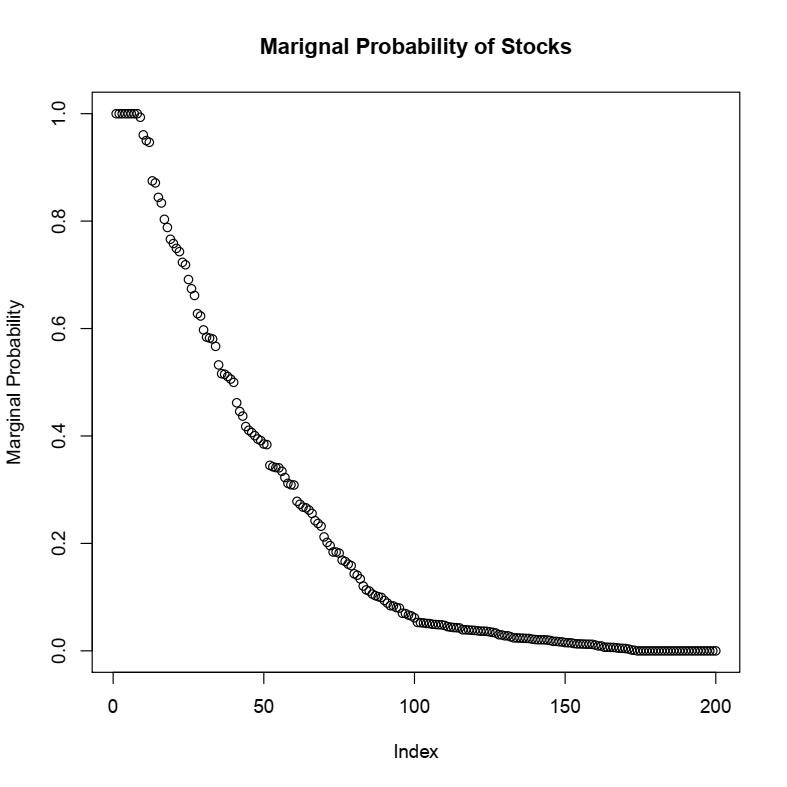
\includegraphics[width=5cm]{colmeans-plot-orig}}
\hfill
\subfigure[Title B]{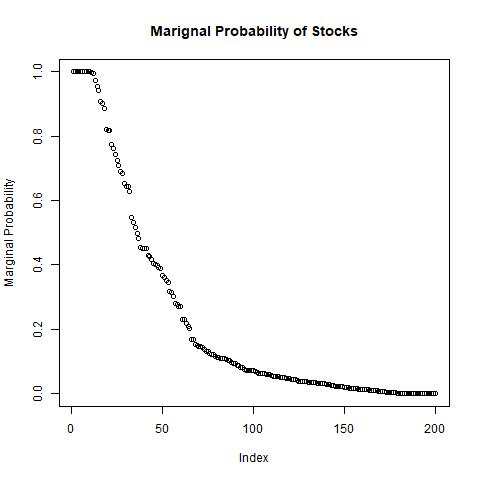
\includegraphics[width=5cm]{colmeans-plot-recent}}
\hfill
\caption{Title for both}
\end{figure}



G\&M continue by running nested regressions and identifying the incremental explanatory power as measured by $R^2$ of each additional candidate stock. Here, we break from G\&M and explore two different measures, in-sample and post tracking error.

{\color{red} Insert plots here for tracking error}
{\color{red} Insert plots here for cumulative returns}

G\&M also makes no comment about the selection of the stocks. For example, looking at those top several stocks that appear to be chosen almost always, do those remain consistent over multiple iterations? Or, particularly due to the correlation structure inherent in the stock market, do we see patterns emerge where highly correlated stocks might be chosen as equivalents?

{\color{red} Insert plots here for distributions by stocks of inclusion probability}



\begin{itemize}
	\item[Optimization]
		\begin{itemize}
		\item Implement Benidis et al. (2018) optimization approaches for setups we find interesting, setups meaning different constraints present on either number of assets or amount held or long-only portfolios, etc.
	\end{itemize}
	\item[Bayesian]
	\begin{itemize}
		\item Extend the basic approach in George and McCulloch (1997) to include portfolio constraints as in Benidis et al. (2018).  The point of this would be to compare to the optimization approaches in Benidis et al. (2018) and see how valuable the Bayesian uncertainty quantification could be.  How much does the optimal solution differ from the posterior?  How wide is the posterior and how far can you get from the optimum while maintaining acceptable performance.
	\end{itemize}
	\item[Gen. fid.]
		\begin{itemize}
			\item Implement Williams and Hannig (2019) approach on index data.
			\item Tweak Williams and Hannig (2019) definition 2.1 of $\eps-$admissibility to account for additional constraints, like those in Benidis et al. (2018).
			\item Compare performance to George and McCulloch (1997), optimization approaches.
	\end{itemize}
\end{itemize}

\subsection{With constraints}

The basic hierarchical model of George and McCulloch (1997) places a normal prior on the asset weights $w$, which does not take into account any type of holding constraints, e.g. long only portfolios.  Here we present an alternative model for long-only portfolios:
\begin{align}
\textbf{r}^b &\sim \nm_{T}(X\textbf{w}, \sigma^2I_{T\times T})\\
\gamma_i &\stackrel{ind.}{\sim} \ber(\alpha_i) \\
\sigma^2 | \gamma & \sim \text{IG}(\nu/2,\,\nu\lambda_\gamma/2)\\
\textbf{w}|\gamma, \sigma^2 & \sim Dir(||\gamma||_0; \beta).
\end{align}
{\color{red} I'm unconvinced it is important to include $\sigma^2$ rather than just set it equal to 1.}

Here the asset weights are given a Dirichlet prior conditional on the included assets.  This prior enforces the constraints $\textbf{w}^\top 1_{N\times 1}=1$ and $\textbf{w}\geq 0_{N\times 1}$.

{\color{blue} It is not obvious how to sample the posterior, which is not of a simple conjugate form.  Most likely, we would use a reversible jump MCMC algorithm.}

\ifthenelse{1=1}{}{
The posterior density $\pi_n$ of $(\gamma, \textbf{w})$ given the data is proportional to the likelihood times the prior density, and can be sampled using, for instance, Metropolis-Hastings within a Gibbs sampler.  Roughly, it would go like this:

\begin{enumerate}
	\item Begin with the $i^{th}$ sample $(\gamma^i, \textbf{w}^i)$.
	\item Propose a new sample of $\gamma$, call it $\gamma^\star$, by drawing it at random from the proposal distribution.  For now, let's say the proposal is Bernoulli with some high probability of $1$ if $\gamma^i_j =1$ and some low probability of $1$ if $\gamma^i_j =0$; such a proposal will tend to slowly change the included assets.
	\item Compute the acceptance ratio (on the log scale):
	\[a=\log \pi_n(\gamma^\star, \textbf{w}^i) - \log \pi_n(\gamma^i, \textbf{w}^i) + \log \pi(\gamma^i) - \log \pi(\gamma^\star)\]
	\item Generate $U\sim \unif(0,1)$ and accept $\gamma^{i+1}=\gamma^\star$ if $\exp(a)>U$.  
\end{enumerate}

A note about computing the ``acceptance ratio": the dimensions of $\gamma^\star$ and $\textbf{w}^i$ may not match, so how should one perform the computation? When computing $\pi_n(\gamma^\star, \textbf{w}^i)$, normalize $\textbf{w}^i$ to the $1$'s indices of $\gamma^\star$.      
}
{\color{red} Not sure what to put here}

However, while theoretically an alternative option to optimization problems, the implementation the reversible jump Markov Chain Monte Carlo requires considerable time to converge. This limitation puts this methodology out of consideration for many portfolio managers.

\section{Conclusion}

In this paper 

{\color{red} discuss additional potential areas of research}
Using the density of the selection to determine regime
Further GFI research
Use of the stocks selected to reduce the parameter set

\section*{References}

\begin{description}

\item{} Benidis, K., Feng, Y., and Palomar, D. P.~(2018). Sparse Portfolios for High-Dimensional Financial Index Tracking. \emph{IEEE Transactions on Sigmal Processing}~66(1), 155-170.

\item{} Fan, J., and Li, R.~(2001). Variable Selection via Nonconcave Penalized Likelihood and its
Oracle Properties. \emph{Journal of American Statistical Association}~96, 1348–1360.

\item{} Fastrich, B., Paterlini, S., and Winker, P.~(2014). Cardinality versus q-norm constraints for index tracking. \emph{Quantitative Finance}~14(11), 2019-2032, DOI: 10.1080/14697688.2012.691986

\item{} Fastrich, B., Paterlini, S. and Winker, P.~(2015). Constructing optimal sparse portfolios using regularization methods. \emph{Comput Manag Sci}~12(3) 417–434. https://doi.org/10.1007/s10287-014-0227-5

\item{} George, E. I., and McCulloch, R. E.~(1997). Approaches for Bayesian variable selection. \emph{Statistica Sinica}~7, 339-373.

\item{} Hastie, D. I. and Green, P. J. (2012), Model choice using reversible jump Markov chain Monte Carlo. Statistica Neerlandica, 66: 309-338. doi:10.1111/j.1467-9574.2012.00516.x

\item{} Puelz, D., Hahn, R. and Carvalho, Carlos M.~(2018). Sparse Mean-Variance Portfolios: A Penalized Utility Approach. \url{https://papers.ssrn.com/sol3/papers.cfm?abstract_id=2729504}.

\item{} Williams, J. P., and Hannig, J.~(2019). Non-Penalized Variable Selection In High-Dimensional Linear Model Settings Via Generalized Fiducial Inference. \emph{Annals of Statistics}.~47(3), 1723-1753. 

\end{description}






\end{document}





